\chapter{Infraestructura Existente}

Conocer la infraestructura disponible es fundamental cuando se debe realizar un diseño, puesto que el diseño debe cumplir con las especificaciones y debe ser compatible con el Hardware. Este proyecto no pretende diseñar piezas mecánicas de construcción del robot, ni confeccionarlas, por lo que el diseño no incluirá esa sección.

En este capítulo se mencionará algunos de los componentes existentes del robot. Por ejemplo, información de los motores, encoders que poseen, la relaciones de engranajes. Se pretende realizar un recuento de los componentes que se utilzarán durante este proyecto, pero que no fueron diseñados propiamente por el proyecto. Esto servirá de guía en los próximos capítulos para el diseño, y la implementación, puesto que los mismos van dirigidos a incorporar todos estos dispositivos en un sólo robot.

En la primera sección, titulada \textbf{Carrito omnidireccional} se discutirá un poco del diagrama de comuniciación básico del proyecto, el cuál justifica el uso de los controladores Roboclaw, y el microcontrolador Stm32f411.

En la sección \textbf{Motores}, se hablará de las especificaciones eĺéctricas y mecánicas de los motores a utilizar, las cuáles serán utilizadas posteriormente en el diseño.

La sección \textbf{Controladores} menciona los controladores de los motores a utilizar, y las funciones relevantes de los mismos que permitirán la conexión con el Stm32f411.

La sección \textbf{Microcontrolador} explica algunas de las funciones del STM32F411 utilizado en este proyecto, y las funciones para leer encoders de cuadratura.

\textbf{Hokuyo} habla de ciertas especificaciones importantes del escaner láser, y finalmente \textbf{Control de PS4} menciona el joystick utilizado posteriormente para mover la base del robot.

\newpage

\section{Carrito omnidireccional}
El ARCOS-Lab tiene varios prototipos de carritos omnidireccionales utilizando ruedas mecanum, los cuáles fueron desarrollados por varios miembros del laboratorio y liderados por Nicole Orosco. Todos los diseños mecánicos de la plataforma, como los soportes de las ruedas, soportes para la batería, para el Kinect, STM32F411 y Raspberry Pi fueron diseñados como parte de otros proyectos de investigación. 

Al momento de iniciar el proyecto, todas las piezas se encontraban impresas y cortadas, además de ensambladas, por lo que sólo fué necesario agregar los componentes que se mostrarán a continuación en la figura \ref{F:diagrama}.

Hay que recoerdar que se requiere de un sistema que pueda controlar los motores, y además llevar control de la odometría de las ruedas. Además se deberá incorporar el sensor de profundidad en el carrito omnidireccional.

\begin{figure}[H]
\centering
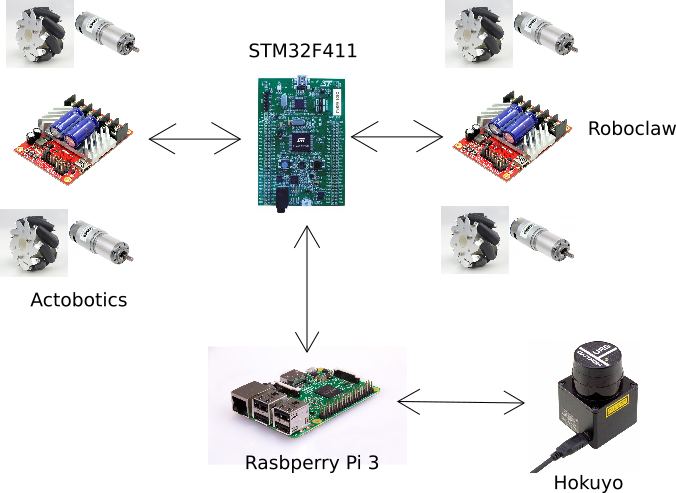
\includegraphics[scale=0.6]{imagenes/diagrama_diseno.png}
\caption{Diagrama básico de la implementación de la parte elétrica del carrito omnidireccional. Autoría propia.}
\label{F:diagrama}
\end{figure}

\section{Motores}

Empezando por los \textbf{motores}, se utilizarán motores DC Actobotics 638276. La hoja de fabricante con los datos en la sección de los apéndices. Además, en la tabla \ref{T:actobotics} se muestra la información más relevante de los motores a utilizar, como por ejemplo el consumo máximo, la tensión de trabajo, y la relación de los engranes.

\begin{table}[H]
\caption{Información más relevante de los motores Actobotics, a ser utilizados. Autoría propia.}
\begin{tabular}{|l|l|}
\hline
Especificación                & Valor         \\ \hline
Voltage de operación          & 6-12 VDC      \\ \hline
Corriente máxima de operación & 0.53 A        \\ \hline
Velocidad máxima sin carga    & 118 $\pm$ 12 rpm \\ \hline
Corriente máxima detenido     & 20 A          \\ \hline
Razón de los engranes         & 1/71          \\ \hline
Clicks del encoder por revolución & 3408      \\ \hline
\end{tabular}
\label{T:actobotics}
\end{table}

Se utilizarán cuatro motores, uno para cada rueda, conectados a ruedas mecanum genericas, de 6mm de diámetro. Estas son ruedas omnidireccionales con rodillos a un ángulo de $\alpha = 45^\circ$.

\section{Controladores}

En lo que concierne a los \textbf{controladores} de los motores, no se diseñarán, puesto que se utilizarán controladores comerciales de marca IonMotion Roboclaw. En específico, se utilizará el modelo Roboclaw 2x15A. En el cuadro \ref{T:roboclaw} se resumen los datos más importantes de este controlador.

\begin{table}[H]
\caption{Información más relevante de los controladores Roboclaw 2x15A. Autoría propia.}
\begin{tabular}{|l|l|}
\hline
Especificación                      & Valor          \\ \hline
Tensión de la batería principal     & 6-34 VDC       \\ \hline
Tensión de la batería lógica        & 6-34 VDC       \\ \hline
Bits de los contadores para encoder & 32 bits        \\ \hline
Velocidad máxima sin carga          & 118 +- 12 rpm  \\ \hline
R232 Baud Rate                      & 460,800 Bits/s \\ \hline
Tensión de I/O                      & 3.3 VDC        \\ \hline
\end{tabular}
\label{T:roboclaw}
\end{table}

Es importante mencionar, que estos controladores se utilizan para manejar los motores. Pueden manejar hasta dos motores, y son muy versátiles en cuánto a cómo se pueden utilizar. En particular, para este proyecto se usará la comunicación serial que posee el controlador. En la figura \ref{F:roboclaw} se muestran los pines que posee el roboclaw. En específico, los pines S1, y S2 se pueden utilizar como puertos USART para comunicación serial. La tabla \ref{T:pines} muestra las funcionalidades que pueden cumplir cada pin.

\begin{figure}[H]
\centering
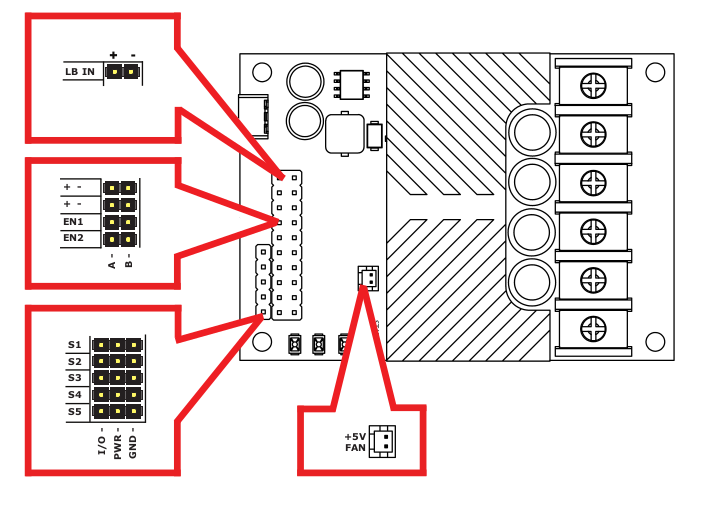
\includegraphics[scale=0.5]{imagenes/roboclaw.png}
\caption{Muestra de los pines de un Roboclaw 2x15A fabricado por IonMotion. Tomado del manual del fabricante.}
\label{F:roboclaw}
\end{figure}

\begin{table}[H]
\centering
\caption{Tabla con las funciones de los pines en un Roboclaw 2x15A fabricado por IonMotion. Tomado del manual del fabricante.}
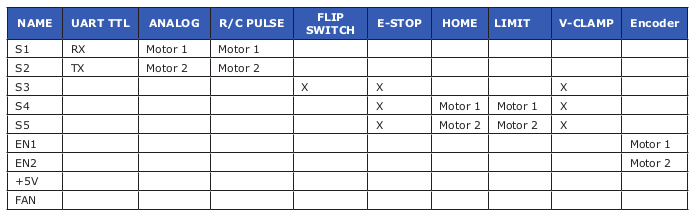
\includegraphics[scale=0.7]{imagenes/pines.png}
\label{T:pines}
\end{table}

Se utilizará una frecuencia de 115200 en la transmisión serial, ya que es la más alta soportada por .

\section{Sistema de desarrollo}

Siguiendo el esquema de la figura \ref{F:diagrama}, los controladores Roboclaw van conectados al \textbf{sistema de desarrollo} STM32F411DISCOVERY, el cuál es manejado por un \textbf{microcontrolador} STM32F411. La principal función de este microcontrolador será llevar cuenta de la odometría de cada una de las ruedas, y del robot como tal. Además, este aceptará instrucciones por USB del Raspberry Pi, de movimiento en el formato $(V_X, V_Y, W_Z)$ y enviará información de vuelta de la odometría del robot en el formato $(X_X, X_Y, \alpha_Z)$. También enviará instrucciones de movimiento a los dos controladores Roboclaw, y controlará la velocidad de cada motor por medio de un PID, en lazo cerrado con la información del encoder como entrada.

El esquema mostrado en la figura \ref{F:diagrama_stm} muestra en resumen lo que se explicó anteriormente.

\begin{figure}[H]
\centering
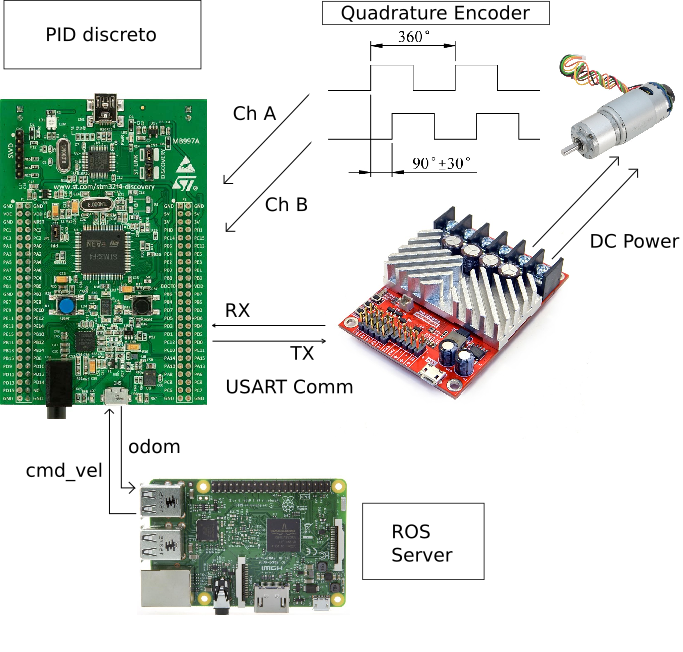
\includegraphics[scale=0.5]{imagenes/microcontrolador_diagrama.png}
\caption{Diagrama de las funciones que debe realizar el microcontrolado STM32F411. Autoría propia.}
\label{F:diagrama_stm}
\end{figure}

Es importante notar, que la programación del microcontrolador se realizará mediante las liberías libopencm3 y libopencm3-plus, las cuáles permiten escribir el código en el lenguaje de programación C. Además, el microcontrolador posee las funciones para leer los encoders directamente, puesto que posee timers que se pueden configurar en un modo para leer codificadores de cuadratura.

Información sobre el uso de encoders de cuadratura en el stm se puede encontrar en apéndice correspondiente.

\section{Hokuyo}

El Hokuyo URG-04LX-UG01 RangeFinder es un sensor de alta calidad y precisión diseñado para realizar escaneos dos dimensionales con un sensor láser. Algunas de las especificacinoes del sensor se encuentran en la tabla \ref{T:hokuyo}. Adicionalmente, la figure \ref{F:hokuyofoto} muestra la fotografía de un sensor Hokuyo.

\begin{table}[H]
\caption{Especificaciones del sensor Hokuyo. Autoría propia.}
\begin{tabular}{|l|l|}
\hline
Especificación       & Valor         \\ \hline
Distancia de escaneo & 20mm a 5600mm \\ \hline
Región de escaneo    & $240^\circ$           \\ \hline
Duración de escaneo  & 100ms/scan    \\ \hline
Resolución angular   & $0.36^\circ$ \\ \hline
Peso aproximado & 160g \\ \hline
\end{tabular}
\label{T:hokuyo}
\end{table}

\begin{figure}[H]
\centering
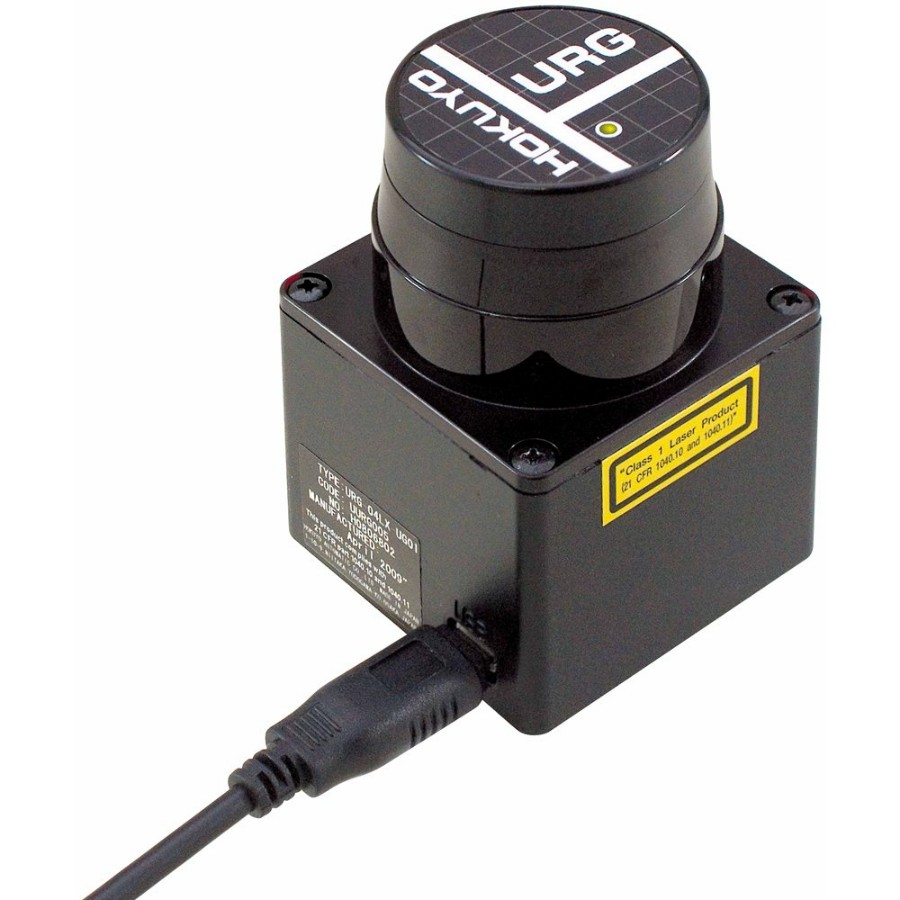
\includegraphics[scale=0.3]{imagenes/hokuyo.jpg}
\caption{Imagen de un ejemplo del sensor Hokuyo, tomado de la página de ventas robotshop.com.}
\label{F:hokuyofoto}
\end{figure}

\section{Control de PS4}

Se utilizará un control de Play Station 4 para mandar comandos de movimiento hacia la base, y realizar pruebas. Los controles de PS4, también conocidos como DualShock4. En la figura \ref{F:dualshock} se muestra una figura del control.

\begin{figure}[H]
\centering
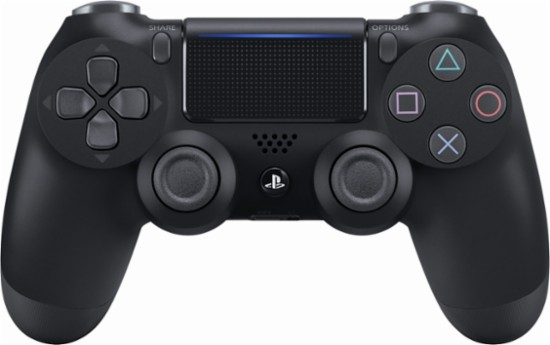
\includegraphics[scale=0.5]{imagenes/dualshock4.jpg}
\caption{Imagen de un control de PS4 dualshock. Tomado de la página de ventas BestBuy.com}
\label{F:dualshock}
\end{figure}

